\documentclass[11pt]{article}

\usepackage{pdfpages}
\usepackage{hyperref}
\usepackage{enumerate}
\usepackage{listings}

\renewcommand*\ttdefault{lmtt}
\renewcommand*\sfdefault{lmss}
\renewcommand{\familydefault}{\sfdefault}

\begin{document}

\author{Hao Chi KIANG}
\title{Laboratory Work 1}
\maketitle

\section{Assignment 1}
The result of all the manipulation in Inkscape are as following.

\begin{figure}[ht]
  \centering
  \includegraphics[scale=0.5]{ass1_plot.pdf}
\end{figure}



\section{Assignment 2}

\begin{figure}[ht]
  \centering
  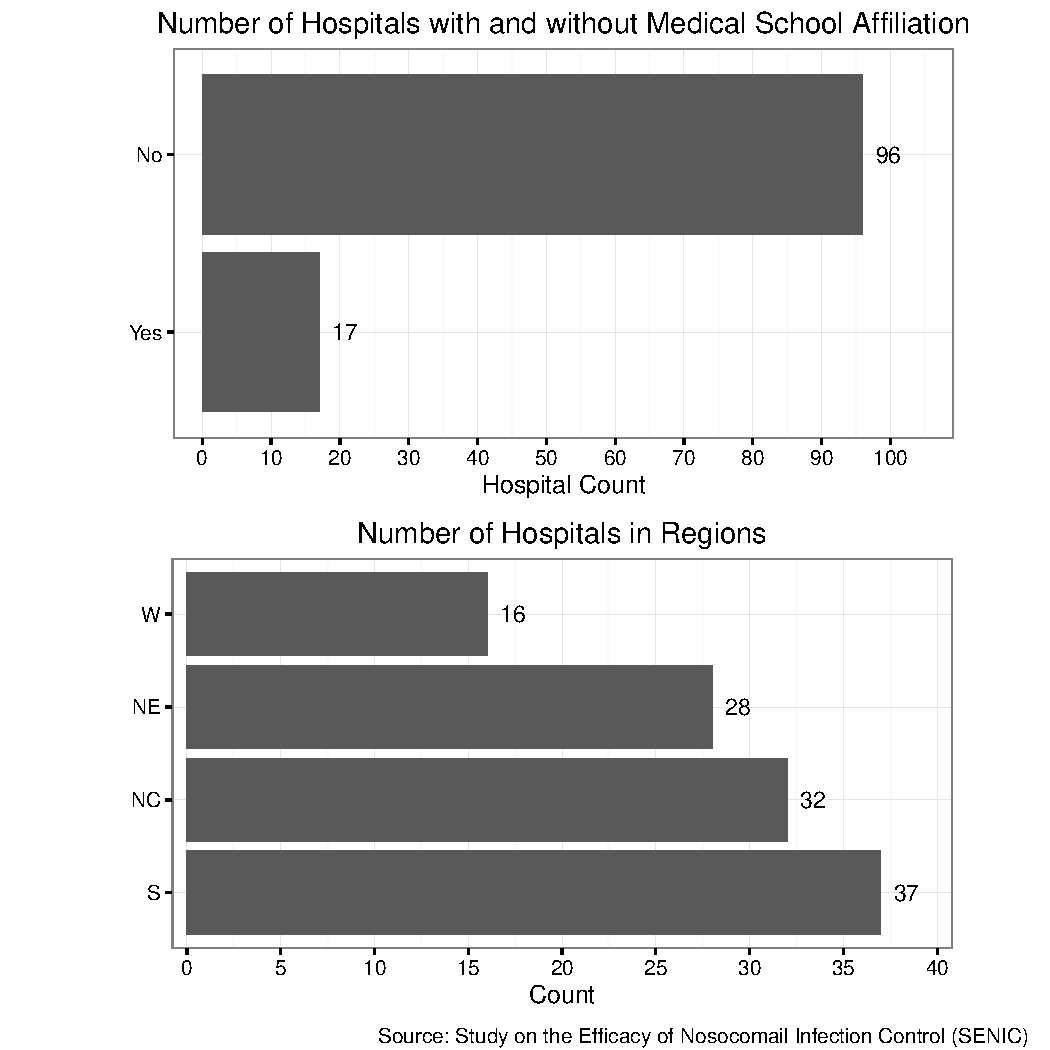
\includegraphics[scale=0.55]{qualitative_vars.pdf}
  \caption{Count of observations of the two
    qualitative variables}\label{fig:qualivars}
\end{figure}

There are only two qualitative variables among all: the Medical School
Affiliation (X7) and Region (X8). \autoref{fig:qualivars} is the combined
chart requested.

We can observe from \autoref{fig:qualivars} that
\begin{enumerate}
\item
  Only a few hospitals have affiliation with medical schools.
\item
  The number of hospital in a region varies a lot across regions. This
  does not tell us anything meaningful, however, unless this count is
  normalized by the population size of each regions. So if this is an
  real analysis, the next step may be to construct a graph of the ratio
  'hospital number/population-size', or even better
  'number of bed/population-size'.
\end{enumerate}


\begin{figure}[ht]
  \centering
  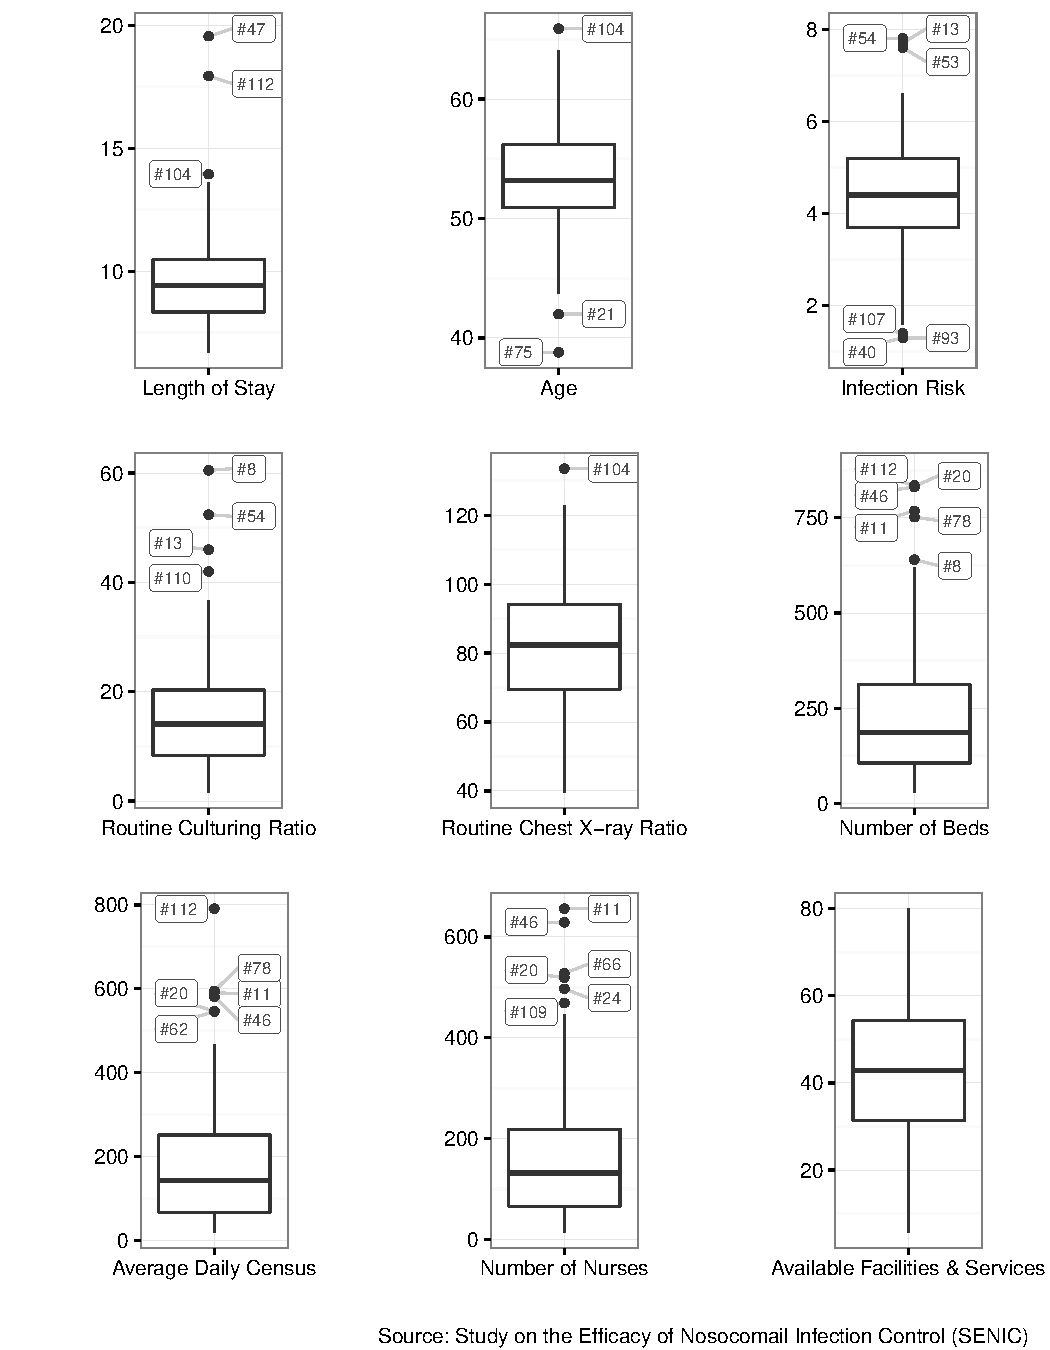
\includegraphics[scale=0.8]{quantitative_vars.pdf}
  \caption{Combined plot of all quantitative variables}\label{fig:quantvars}
\end{figure}

The quantitative variables are plotted in box plots in \autoref{fig:quantvars}.

The following are some observations:
\begin{enumerate}
\item
  Average length of stay varies among the hospitals from less than five days to
  near 20 days. This suggest that some hospitals does not have bed or service of
  taking many long-staying patients.
\item
  Both number of nurses, average daily census and number of beds ranges from
  several dozens to several hundreds. They also shares many outliers. This suggest
  some hospitals are having many staying patients and some hospitals doesn't take
  in many staying patients at all.
\item
  Hospital \#104 outlies in both length of stay and average age of patient. It
  seems that this hospital probably has a geriatric or paliative care service.
  Its outlying in routine chest X−ray ratio may be related to this as well.
\item
  Hospital \#13 and \#54 outlies together in both infection risk and routine culturing
  ratio. Both intuition and this coincidence leads us to suspect there is corelation
  between culturing and infection. Ploting them in a scatter plot may help us find
  this out.
\end{enumerate}




\section{Assignment 3}

\subsection{Nurse-to-bed ratio}
\label{subsec:nurse2bed}
\lstset{
  frame=single,
  basicstyle=\ttfamily\footnotesize,
  commentstyle=\color{gray},
  language=R,
}

\begin{lstlisting}[caption={Hospital with the lowest nurse-to-bed ratio}\label{lst:leastnurse}]
least_nurse_hospital <-
    senic_data[which.min(senic_data$X10/senic_data$X6),]

# Result:
#     Obs   X1   X2  X3  X4   X5  X6 X7 X8 X9 X10  X11
# 107 107 7.14 51.7 1.4 4.1 45.7 115 No  S 90  19 22.9
\end{lstlisting}


\autoref{lst:leastnurse} gives the hospital with the lowest nurse-to-bed ratio.
Hospital \#107 has 115 beds but only 19 nurses. The ratio is 0.165. This ratio
shows on average how many nurses a bed has. Staying patient should be better off
when this ratio is bigger. Nurses seem to be short-staffed in this hospital.


\subsection{Infection risk versus Identification number}

\begin{figure}
  \centering
  \includegraphics[scale=0.8]{infection_risk_ANCOVA.pdf}
  \caption{Infection risk vs. Identification number, with predicted values. The red
    point is the \#107 mentioned in \autoref{subsec:nurse2bed} }
  \label{fig:infection_risk}
\end{figure}

\autoref{fig:infection_risk} is a scatter plot of infection\_risk verses identification number.
The hospital \#107 with worst nurse-to-bed ratio has very low infection risk, which is an
unexpected observation. Although this hospital is particularly at the corner of the
plot, without enough information of how the hospital identification number is assigned,
we cannot simply conclude that either infection risk or nurse-to-bed ratio has any relationship
with identification number.

The regression done between infection risk and identification number simply fails to predict
the infection risk by identification number, as points are so away from the prediction line
and the prediction gives something near the mean no matter what identification number it is.
The slightly declining trend seems to be just the effect of that all three upper outliers
are having their identification number less than 60.

Despite all this, I would choose not to conclude that the identification numbers are given
randomly. They can still be corelated to variables that are not captured in the data set.
We can only conclude from the graph that identification numbers are not corelated to
infection risk, but not other any variables.

\section{Full Code and Figures}
All the codes and figures in the report should be included in the same ZIP file.

\end{document}
